Mes travaux de thèse s'appuient sur des comparaisons de paysages de régulation de l'expression des gènes. Il m’est donc nécessaire de commencer par préciser les notions dont il est question : gènes, expression, régulation, éléments régulateurs, et les techniques de mesure de leur existence ou de leur quantité. Je m’attarderai sur certaines techniques et méthodologies qui ont permis de prédire et mesurer ces objets, avant de contextualiser les connaissances actuelles sur leur évolution et leurs relations, qui ont été le point de départ de ma thèse.

\chapter{L’expression des gènes}
{\hypersetup{linkcolor=GREYDARK}\minitoc}
\label{chap:expression-des-gènes}

\section{Définitions}
\label{sec:definition-des-gènes}

La notion de gène dépend grandement des besoins et des usages qu’on en fait, et sa définition a largement évolué au cours de la compréhension de la complexité moléculaire de l’\acrshort{ADN} \citep{gerstein_what_2007}. D’abord unité de trait héritable \citep{mendel_verhandlungen_1866}, puis région du génome à l’origine d’une protéine \citep{morgan_mechanism_1915,beadle_genetic_1941}, le gène a ensuite été caractérisé comme une séquence précise de l’\acrshort{ADN} \citep{watson_molecular_1953}, qui doit être transcrite puis traduite selon un code génétique pour être fonctionnelle et affecter les caractères d’un organisme \citep{nirenberg_rna_1965}. L’émergence et le développement des techniques de séquençage ont par la suite permis de préciser la structure des gènes en annotant notamment les parties codantes (exons) et non-codantes (promoteur, introns, extrémités), ce qui a rendu possible la prédiction et la détection d’autres catégories de gènes \citep{fiers_complete_1976, doolittle_urfs_1986}. Il est cependant rapidement apparu que l’idée “qu’un gène produit une protéine” était une simplification excessive. Premièrement, la présence de nombreux gènes transcrits en \acrshort{ARN}s directement fonctionnels sans être traduits et ne codant donc pas pour des protéines n'est pas en accord avec une telle idée \citep{lander_initial_2001}. Deuxièmement, le développement de techniques de séquençage à haut débit a révélé la complexité du transcriptome \citep{birney_identification_2007, encode_project_consortium_integrated_2012}. Que ce soit pour les gènes codants pour des protéines ou pour certains gènes non-codants (pour des \acrshort{ARN}s), l’\acrshort{ARN} subit une maturation pour être stabilisé et fonctionnel, notamment un épissage qui consiste à exciser les parties introniques des transcrits pour conserver les exons. Cet épissage peut être variable en retenant certains introns ou en excisant certains exons et peut ainsi produire des transcrits alternatifs pour un même gène. De plus, la transcription d’un gène peut démarrer à partir de sites d’initiation alternatifs engendrant également des transcrits différents. Pour les gènes codants, ces transcrits alternatifs peuvent conduire à différentes versions de protéines appelées isoformes et pouvant avoir des fonctions différentes. La délimitation d’un gène comme unité peut alors être délicate, notamment par le fait que les gènes peuvent se chevaucher et ainsi avoir des parties fonctionnelles en communs. J’utiliserai au cours de cette thèse la définition d’un gène comme étant une séquence d’\acrshort{ADN} qui est transcrite pour produire une molécule pouvant impacter les caractères phénotypiques de l’organisme. \\

Les gènes peuvent produire une quantité variable de produits finaux (protéines ou \acrshort{ARN}s non-codants matures) qui sont potentiellement fonctionnels dans la cellule et plus largement dans l’organisme. Il peut alors être nécessaire de quantifier cette activité, définie comme le niveau d'expression d’un gène, pour estimer son impact. La quantité des produits finaux est cependant difficilement accessible pour de nombreux gènes, notamment ceux codant des protéines. En effet, ces dernières présentent une grande diversité d’abondance mais surtout de structure de par leur constitution en acides aminés et leur conformation tridimensionnelle leur donnant des propriétés biochimiques distinctes. C’est par exemple le cas des protéines trans-membranaires, présentes en très faible quantité et difficilement solubles \citep{vuckovic_membrane_2013}. Les protéines réagissent de manière très diverse aux protocoles expérimentaux et la capture, l’isolation et l’identification de l’ensemble des protéines d’une cellule est très complexe. A ce jour, l’identification des protéines chez humain n’est ainsi toujours pas complétée et nécessite la collaboration de plusieurs centaines d'équipes dans le monde, via le consortium Human Proteome Project, depuis plus de 10 ans \citep{adhikari_high-stringency_2020}. Il est néanmoins possible d’approximer le niveau d’expression d’un gène en mesurant la quantité d’\acrshort{ARN} messager produit lors de sa transcription. Il est en effet plus simple d’isoler et de séquencer l’\acrshort{ARN} messager, composé seulement de quatre nucléotides distincts, que les protéines. Les techniques de séquençage de l’\acrshort{ARN}, dites \acrshort{RNA-seq}, permettent de mesurer la quantité d’\acrshort{ARN}s matures, à l’état stable, et donc après modifications post-transcriptionnelles \citep{chu_rna_2012}. Il a été montré que cette mesure de la quantité d’\acrshort{ARNm} stable d’un gène codant est bien corrélée à la quantité de ses protéines produites dans une cellule \citep{edfors_gene-specific_2016}. L’utilisation du \acrshort{RNA-seq} est aujourd’hui largement répandue et permet de donner une définition plus usuelle du niveau d’expression des gènes comme étant le nombre de molécules d’\acrshort{ARNm} produites par le gène, par cellule, tous transcrits alternatifs confondus. Enfin, un des avantages notables du séquençage d’\acrshort{ARN} est la possibilité d'identifier des nouveaux transcrits et de quantifier l’expression des gènes ne codant pas pour des protéines. \\

Afin d’illustrer mes propos le long de cette introduction, je reviendrai régulièrement sur l’exemple du gène Sonic hedgehog, qui est devenu un modèle pour comprendre les fonctions d’un gène, son expression, sa régulation, mais aussi son évolution. Le gène hedgehog est un gène codant identifié d’abord chez la drosophile pour son rôle crucial dans la segmentation lors du développement embryonnaire \citep{nusslein-volhard_mutations_1980}. Chez les vertébrés ce gène est présent en trois copies, dites homologues, qui ont émergé suite à deux duplications successives du génome complet chez l’ancêtre commun du clade et par la perte d’une copie \citep{dehal_two_2005}. L’expression de ces trois gènes permet notamment de définir la voie de signalisation Hedgehog qui joue plusieurs rôles majeurs lors du développement embryonnaire, comme l’organogénèse, l’organisation du cerveau ou le développement de structures comme les doigts \citep{lum_hedgehog_2004}. L’un de ces homologues les plus étudiés est Sonic hedgehog (\acrshort{SHH}) localisé sur le chromosome 7 chez l’humain. Le niveau d’expression de \acrshort{SHH}, et donc la quantité de la protéine \acrshort{SHH} dans les cellules, permet de définir un gradient de concentration qui va contrôler l’expression de plusieurs autres gènes. Dans le développement des membres par exemple, le gradient de concentration de cette protéine, dans une zone dite de polarisation, est essentiel pour établir un axe antéro-postérieur permettant de définir le nombre et la structure des doigts (Figure \ref{fig:Fig1}) \citep{riddle_sonic_1993, echelard_sonic_1993}.

\begin{figure}[h]
    \centering
    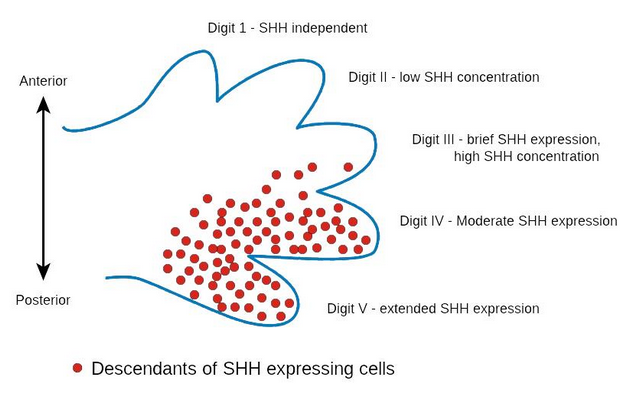
\includegraphics[width=1\textwidth, page=1] {figures/introduction/fig1.png}
    \caption[Schéma de l'impact de l'expression de \acrshort{SHH} au cours du développement d'un membre.]{
    \textbf{Schéma de l'impact de l'expression de \acrshort{SHH} au cours du développement d'un membre.} Le gradient de concentration de la protéine \textit{Shh} dans la zone d'activité polarisante (ZPA) dans le bourgeon du membre permet de définir un axe antéro-postérieur.  Les cellules déterminées par la signalisation SHH
permettront la formation des os postérieurs de l'autopode et du zeugopode.  Tirée de \citep{lezot_shh_2020}
    }
    \label{fig:Fig1}
\end{figure} 


\section{Mesures et comparaisons de l’expression}
\label{sec:mesure-et-comparaison}

L’expression d’un gène varie selon les stades de développement, les types cellulaires ou les facteurs externes. L’expression des gènes est considérée comme le premier échelon du phénotype moléculaire d’un organisme, qu’il est nécessaire de mesurer indépendamment dans chaque échantillon.

\subsection{RNA-seq et niveau d’expression}
\label{subsec:RNAseq-niveau-expression}
Les méthodes de séquençage à haut débit de l’\acrshort{ARN} (\acrshort{RNA-seq}) permettent d’approximer le niveau d’expression des gènes à un instant donné dans un échantillon. Celles-ci s’effectuent généralement sur une population de cellules, ce qui permet d’obtenir une mesure globale d’un ensemble de transcrits produits ou transcriptome. Grâce au développement récent de techniques microfluidiques permettant d’isoler un très faible nombre de cellules, voire des cellules uniques, la quantification du transcriptome peut désormais se faire à l’échelle d’une seule cellule \citep{tang_mrna-seq_2009}. 
 \\

Les techniques de \acrshort{RNA-seq} passent généralement par cinq grandes étapes : l’isolation de l’\acrshort{ARN}, la sélection/déplétion de certains \acrshort{ARN}s, la transcription réverse en \acrshort{ADN} (essentielle à l’étape d’amplification par PCR), l’amplification puis le séquençage à haut débit. L’étape de sélection/déplétion est cruciale car de nombreuses formes distinctes d’\acrshort{ARN} sont présentes dans les cellules. Les \acrshort{ARN}s ribosomaux par exemple, qui sont non codants et permettent la synthèse des protéines, représentent une très grande partie du contenu en \acrshort{ARN} d’une cellule (plus de 80\%) et doivent généralement être filtrés \citep{oneil_ribosomal_2013}. Il est possible de cibler spécifiquement certains types d'\acrshort{ARN}s. Par exemple, les \acrshort{ARN}s messager matures des gènes codants pour des protéines contiennent une séquence terminale poly-A, tout comme certains longs \acrshort{ARN}s non-codants. Ces transcrits peuvent être ciblés en passant par une étape d'hybridation avec des molécules poly-T se liant de manière covalente à la queue poly-A. Il est également possible de viser les petits \acrshort{ARN}s non-codants, tels que les micro\acrshort{ARN}s, piwi\acrshort{ARN}s, etc, en filtrant les transcrits selon leur taille. Certaines techniques dérivées permettent de sélectionner d’autres formes d’\acrshort{ARN}, comme les \acrshort{ARN}s en cours de transcription (ou \acrshort{ARN}s naissants) qui reflètent directement le taux de transcription des gènes \citep{core_nascent_2008}. 

\subsection{Tests d’expression différentielle}
\label{subsec:expression-différentielle}

Il peut être intéressant de comparer le niveau d’expression d’un gène entre différentes \glspl{condition} biologiques, pouvant être des types cellulaires distincts, des stades du développement, une réponse à un stimulus, ou encore des comparaisons entre individus ou espèces. Cependant ces comparaisons peuvent être complexes, notamment car la quantité d’\acrshort{ARNm} est une variable discrète pouvant fluctuer entre zéro et des valeurs extrêmement hautes de concentration, et qui peut être composée d’une part non négligeable de “bruit”. Il est également nécessaire de corriger les biais techniques inhérents aux méthodes de séquençage. Deux facteurs sont en effet essentiels à prendre en compte : le nombre de lectures de l’\acrshort{ADN} qui sont séquencées et la longueur des exons que celles-ci couvrent sur le génome. Le premier paramètre définit la profondeur de séquençage et influence directement le nombre de lectures attribuées à chaque \acrshort{ARN} messager (\acrshort{ARNm}). Le second paramètre reflète la taille des \acrshort{ARNm} séquencés qui est principalement déterminée par le nombre et la taille des exons de l’organisme étudié. La taille des lectures de séquençage étant généralement fixe et définie par le protocole, un transcrit plus long va générer un plus grand nombre de lectures qu’un transcrit court du même niveau d’expression. Une étape de normalisation est alors nécessaire. Une définition possible de la mesure du niveau d’expression d’un gène peut alors être le nombre de lectures associé à ses \acrshort{ARNm} divisé par sa longueur exonique exprimée en kilobases et par million de lectures séquencées (\acrshort{RPKM}) prenant ainsi en compte à la fois la taille du transcrit et la profondeur de séquençage. En \acrshort{RNA-seq}, la mesure du niveau d’expression d’un gène ne représente pas un nombre absolu de molécules mais est une proportion relative à l’expression des autres gènes. Avec les techniques classiques de RNA-seq la comparaison entre deux échantillons quelconques ayant les mêmes proportions d’abondance entre les transcrits, mais dont la quantité totale d’\acrshort{ARN} est différente, ne montrera pas de différence significative d’expression. \\

Les tests de comparaison des niveaux d’expression font l’hypothèse que la médiane des niveaux d’expression sur tous les gènes est la même entre les échantillons \citep{robinson_edger_2010, love_moderated_2014}. Or, cette hypothèse n’est pas respectée en mesurant le niveau d’expression des gènes par \acrshort{RPKM} \citep{wagner_measurement_2012}. En effet cette mesure étant à l’échelle des lectures de séquençage, dans un échantillon contenant des transcrits plus long le même nombre de lectures représentera moins de transcrits. Une autre métrique, le nombre de transcrits d’un gène par million de transcrits séquencés (TPM), définit à l’échelle des transcrits et non plus des lectures, permet de corriger ce biais \citep{wagner_measurement_2012}. Il assure notamment que la moyenne des niveaux d’expression des gènes mesurée sur une annotation de transcrits identiques est strictement égale entre échantillons. C’est grâce à cette normalisation qu’il est possible de comparer rigoureusement les niveaux d’expression des gènes entre plusieurs échantillons d’une même espèce. Cependant il peut être beaucoup plus délicat de comparer le niveau d’expression entre espèces distinctes, d’autant plus que leur distance phylogénétique est importante. Premièrement, la principale limitation est qu’en raison de contraintes physiologiques engendrant une quantité totale d’\acrshort{ARN} différente par cellule, l’hypothèse d’égalité des niveaux moyens (ou médians) d’expression des gènes n’est pas garantie. Ainsi les niveaux d’expression des gènes tels que mesurés par \acrshort{RPKM} ou TPM sont difficilement comparables directement, sans précautions supplémentaires. Deuxièmement, les lectures de séquençage \acrshort{RNA-seq} doivent être associées à un répertoire de gènes orthologues entre les espèces. La définition des relations évolutives entre les gènes d’espèces distinctes, c'est-à-dire leur similarité de structure (homologie) et leur provenance d’un même gène ancestral par spéciation (orthologie), n’est pas une question triviale. De plus, l'estimation des niveaux d'expression des gènes n’étant pas basée sur les mêmes annotations ou les mêmes ensembles de transcrits, un nombre variable de transcrits alternatifs associés à un même gène pourra biaiser la comparaison entre deux espèces. Les différences de qualité d'annotations sont systématiques même entre les deux espèces modèles que sont l’humain et la souris. Pour limiter les biais, il est possible de prendre en compte des annotations rigoureusement identiques à partir par exemple d’un ensemble commun d’exons alignés entre espèces. La normalisation des niveaux d’expression au sein de chaque espèce par rapport aux gènes dont l’expression varie le moins (les gènes "de ménage") peut également être utile \citep{brawand_evolution_2011}.

\subsection{Patrons d’expression}
\label{subsec:Patron-expression}

Le patron d’expression d’un gène, c’est-à-dire son activité ou son niveau d’expression dans l’ensemble des types cellulaires, tissus ou des stades de développement d’un organisme est une mesure pertinente pour des comparaisons inter-espèces. Plutôt qu’une différence quantitative évaluée dans une seule condition, la comparaison des patrons d’expression peut renseigner sur des changements plus importants comme des gains ou des pertes d’activité d’un gène dans un tissu ou à un stade de développement, des changements de dynamique temporelle etc.  \\

Le patron d’expression peut être approximé par le niveau d’expression d’un gène dans un nombre limité de \glspl{condition}, que nous allons appeler ci-dessous un profil d’expression. En utilisant non pas les valeurs absolues des niveaux d’expression d’un gène mais plutôt leurs valeurs relatives entre les échantillons, obtenues par exemple en divisant par le maximum (ou la somme) des niveaux d'expression, il est possible de faire des comparaisons entre espèces. Ces profils relatifs permettent de s’affranchir de l’hypothèse d’égalité des niveaux d’expression médians. Il est cependant essentiel d’évaluer le profil d’expression dans des échantillons comparables entre espèces : par exemple, les mêmes tissus aux stades de développement comparables, ou bien des types cellulaires comparables. Ces profils peuvent révéler des différences qualitatives des changements d’expression d’un gène. L’analyse des profils relatifs d'expression de l’humain et de la souris permet par exemple d’observer des trajectoires temporelles de l'expression du gène \acrshort{SHH} divergente au cours du développement du foie et du coeur (Figure \ref{fig:Fig2}). Cette transformation permet d’effectuer des analyses évolutives que j’aborderai un peu plus tard (\ref{subsub:evol-profil}). C’est notamment en comparant des profils d’expression relatifs entre humain et souris que j’ai pu effectuer le travail présenté en Chapitre 3 (\ref{part:chap3}. \\

\begin{figure}[h]
    \centering
    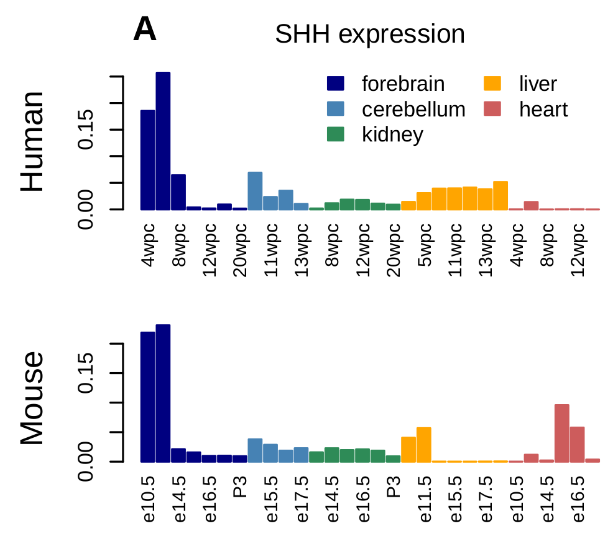
\includegraphics[width=0.8\textwidth, page=1] {figures/introduction/fig2.png}
    \caption[Profils d'expression relatifs du gène \acrshort{SHH} chez l'humain et la souris.]{
    \textbf{Profils d'expression relatifs du gène \acrshort{SHH} chez l'humain et la souris.}
    Les données d'expression proviennent de différents tissus obtenus à des stades de développement comparables \citep{cardoso-moreira_gene_2019}. La correspondance entre les stades de développement est tirée de la publication d'origine.\\
    }
    \label{fig:Fig2}
\end{figure} 

Le patron d’expression d’un gène permet également de mesurer l’étendue de son expression, c’est-à-dire le nombre de tissus/stades de développement/types cellulaires dans lesquels il est actif. On peut également parler de la spécificité d’un gène qui correspond à l’inverse de son étendue. Le patron d’expression peut ainsi révéler des gènes constitutifs, exprimés dans quasiment toutes les cellules comme c’est le cas des gènes de ménage, ou à l’inverse des gènes très spécifiques d’un tissu ou d'un type cellulaire. L’expression d’un gène dans plusieurs conditions peut être l’indication d’une multiplicité de ses fonctions, le gène peut agir sur plusieurs caractères et est alors qualifié de pléiotrope.

\section{Variations de l’expression et conséquences sur les phénotypes}
\label{sec:variations-et-consequence}

L’analyse des patrons d’expression des gènes permet d’observer de grandes variations d’activité entre différents tissus ou types cellulaires d’une même espèce. Ces variations de l’expression des gènes reflètent des fonctions biologiques bien distinctes entre les tissus et/ou les stades de développement de l’organisme, et permettent notamment aux cellules de se spécialiser dans différentes fonctions. \\

Des changements du patron d’expression d’un gène, par son activation ou son inactivation dans un tissu, peuvent avoir des conséquences importantes sur l’organisme. Il est possible d'étudier l’effet de tel changement du patron d’expression en inactivant localement un gène ou en induisant artificiellement un changement de son expression. Une telle expérimentation a été faite pour l’expression du gène \acrshort{SHH} chez l’axolotl, une espèce qui a la capacité de régénérer ses membres lorsqu’ils sont sectionnés \citep{roy_vaccinia_2000}. Dans cette étude, un virus \textit{Vaccinia} modifié pour exprimer le gène \acrshort{SHH} a été injecté dans la partie antérieure des membres en régénération. L’expression anormale de \acrshort{SHH} qui en résulte entraîne de sévères malformations des membres, avec un nombre surnuméraire de doigts et de phalanges (Figure \ref{fig:Fig3}). \\

\begin{figure}[h]
    \centering
    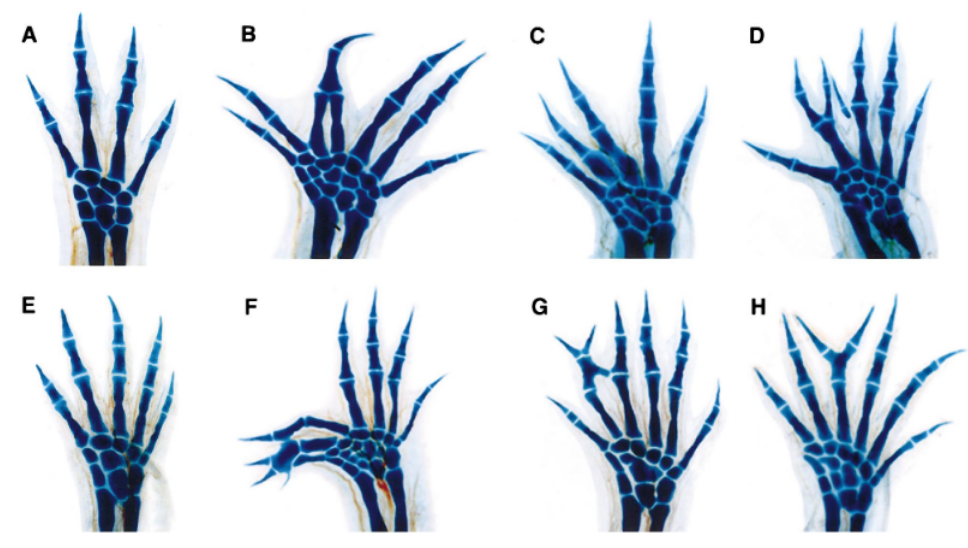
\includegraphics[width=0.8\textwidth, page=1] {figures/introduction/fig3.png}
    \caption[Radiographies de squelettes régénérés de membres antérieurs et postérieurs d'axolotls avec ou sans injection d'un virus Vaccinia exprimant le gène \acrshort{SHH}.]{
    \textbf{Radiographies de squelettes régénérés de membres antérieurs et postérieurs d'axolotls avec ou sans injection d'un virus Vaccinia exprimant le gène \acrshort{SHH}} \textbf{A et E} :  Régénération normale d'un membre antérieur et postérieur chez un axolotl sans injection. \textbf{B-D} :  Régénération d'un membre antérieur après injection, présentant des doigts et des carpiens supplémentaires. \textbf{F-H} : Régénération d'un membre postérieur après injection, présentant des doigts et des tarses supplémentaires. Tirées de \citep{roy_vaccinia_2000}.\\
    }
    \label{fig:Fig3}
\end{figure} 

Ces conséquences soulignent l’importance de la régulation spatio-temporelle de l’expression des gènes dans l'établissement des phénotypes des organismes.
